% ---------------------------------------------------------------------------
% Springer LNCS build.  Compile with:
%     tectonic -X compile main.tex --outdir .
% The body is shared verbatim with ../ieee/main.tex; only this wrapper differs.
% ---------------------------------------------------------------------------
\documentclass[runningheads]{llncs}

\usepackage{graphicx}
\usepackage{booktabs}
\usepackage{amsmath}
\usepackage{amssymb}
\usepackage{siunitx}
\usepackage{microtype}
\usepackage[hidelinks]{hyperref}

\graphicspath{{../shared/generated/}}

% siunitx v3 dropped \degree; every bare (non-\si) use in the body is in math
% mode.
\providecommand{\degree}{^{\circ}}

% LNCS is single-column, so a "wide" float is just a normal float.
\newenvironment{wfigure}{\figure}{\endfigure}
\newenvironment{wtable}{\table}{\endtable}
\newcommand{\tabscale}{\footnotesize}

% llncs sets a run-in \paragraph with no trailing punctuation of its own, so
% the period belongs here. IEEEtran appends its own colon and must not get one.
\newcommand{\para}[1]{\paragraph{#1.}}

% llncs uses \cite, not natbib's \citep. Map it so the shared body compiles
% unchanged under both classes.
\providecommand{\citep}[1]{\cite{#1}}

% Every experimental number in the prose is a macro; see the header comment
% in shared/generated/macros.tex for its provenance and evidence grade.
% ---------------------------------------------------------------------------
% Numeric macros used by shared/body.tex. Every number below was read directly
% from backend/services/sst_anomaly.py's module docstring (verified in full,
% all 209 lines, on \AsOf{}), cross-checked against DONE.md's "A rolling wind
% history" entry (2026-08-28) for the third experiment, and against the source
% constants named per group. None of this was copied from research/research.md
% \S1.12 or from research/papers/silent_failures/ — those documents are
% treated as pointers, not sources, per this project's own house rule after
% two prior research.md errors were found this session. Concretely:
%   - research.md's \S1.12 states the per-cell disagreement's "no systematic
%     offset" claim as "mean +0.005 degC over 60S-60N". That figure appears
%     nowhere in sst_anomaly.py's own docstring, which gives a per-cell mean
%     of +0.033 degC (open ocean) and +0.131 degC (coastal band) -- two
%     different numbers, neither +0.005. +0.005 is not used anywhere below.
%   - research.md's \S1.12 does not mention the matched-GLORYS-climatology
%     attempt (2026-08-25) or the rolling-wind-history attempt (2026-08-28)
%     at all; both are documented directly in sst_anomaly.py's docstring and
%     in DONE.md, dated after research.md's own last revision on this topic.
%
% Evidence grade for every number in this file: DATED. Every measurement is a
% single, live run against a moving field (a day's wind/currents/SST state),
% named with its date and its reproduction script, with no stored output file
% committed anywhere in the repository. The three reproduction scripts
% (measure_sst_corroboration.py, build_climatology_copernicus.py,
% measure_wind_history_corroboration.py) plus backfill_wind_history.py and
% services/wind_history.py ARE committed and were confirmed to exist and to
% do what this file describes -- so the correct grade is "reproducible on
% demand from a committed script, no stored output," which is stronger than
% "no evidence" and weaker than the Artifact grade silent_failures reserves
% for a committed report or currently-passing test. Nothing here should be
% read as a standing fact about the current state of any live field.
% ---------------------------------------------------------------------------

\newcommand{\AsOf}{2026-09-09}
\newcommand{\NCrossProductFixes}{2}

% --- Fixed thresholds and baseline windows the two tests are built on ---
% backend/services/upwelling.py:169, COOL_ANOMALY_C = 0.5 (the weak tier's
% fixed absolute anomaly threshold).
\newcommand{\CoolAnomalyThreshold}{0.5}
% backend/services/climatology/build.py: PERCENTILES = (10, 90) (line ~72);
% DEFAULT_WINDOW_DAYS = 5 (day-of-year pooling half-width, line 67). The cold
% (10th) percentile is what the strong tier actually tests against
% (services/sst_anomaly.py's cold_exceedance); the warm (90th) companion from
% the same PERCENTILES tuple is named separately so Hobday et al.'s
% warm/cold pair (\S2) can be stated without gluing a literal "0" onto
% \ClimPercentile{} (that concatenation previously rendered "100th").
\newcommand{\ClimPercentile}{10}
\newcommand{\ClimPercentileWarm}{90}
\newcommand{\ClimWindowDays}{5}
% OISST climatology: build.py DEFAULT_BASELINE_START/END = 1991/2020.
\newcommand{\OisstBaselineStart}{1991}
\newcommand{\OisstBaselineEnd}{2020}
% GLORYS-fitted climatology: scripts/build_climatology_copernicus.py
% DEFAULT_BASELINE_START/END = 1993/2022 -- the longest 30-year window the
% reanalysis's 1993 coverage start actually supports (its own docstring
% states 1991-2020 is unavailable and build_climatology would reject it).
\newcommand{\GlorysBaselineStart}{1993}
\newcommand{\GlorysBaselineEnd}{2022}
% Copernicus GLORYS reanalysis dataset id, from build_climatology_copernicus.py.
\newcommand{\GlorysDatasetId}{cmems\_mod\_glo\_phy\_my\_0.083deg\_P1D-m}

% --- Fix A: swap the scored observation from OISST to a fresher, higher- ---
% --- resolution live product, holding the climatology fixed [2026-08-17] ---
% sst_anomaly.py docstring, first table. copernicus_sst.anomaly_field() was,
% at this date, implemented to score the live Copernicus physics field
% against the OISST-fitted climatology (services/copernicus_sst.py:210-224's
% own docstring states this configuration directly and that it "was measured
% and made services/upwelling.py's corroboration worse"). Both arms scored
% over the identical live wind/currents snapshot; contrast = favourable minus
% control (downwelling-favourable coastal cells).
\newcommand{\FixAWeakOisst}{0.026}
\newcommand{\FixAWeakLive}{0.022}
\newcommand{\FixAStrongOisst}{0.002}
\newcommand{\FixAStrongLive}{-0.149}

% --- Per-cell product disagreement, measured directly [2026-08-01] ---
% sst_anomaly.py docstring, second table: one day of hourly Copernicus
% physics, daily-averaged and coarsened onto the OISST grid, compared
% cell-by-cell against OISST. Open ocean vs. the coastal band, kept as two
% distinct rows throughout this paper -- do not merge them.
\newcommand{\DisagOpenMean}{0.033}
\newcommand{\DisagOpenMedian}{0.011}
\newcommand{\DisagOpenSD}{0.467}
\newcommand{\DisagOpenFracHalf}{14.3}
\newcommand{\DisagOpenFracOne}{3.9}
\newcommand{\DisagCoastalMean}{0.131}
\newcommand{\DisagCoastalMedian}{-0.002}
\newcommand{\DisagCoastalSD}{0.758}
\newcommand{\DisagCoastalFracHalf}{24.9}
\newcommand{\DisagCoastalFracOne}{10.0}

% --- Fix B: fit a matched climatology on the product being scored ---
% [2026-08-25] sst_anomaly.py docstring, third table. GLORYS-fitted
% climatology built for real by build_climatology_copernicus.py (30 years,
% 1993-2022); copernicus_sst.anomaly_field() was repointed to it
% (REANALYSIS_CLIMATOLOGY_VARIABLE, copernicus_sst.py:207,235) and is the
% version shipped today, though services/upwelling.py's production
% corroboration still consumes heatwaves.sst_anomaly_field() (OISST), not
% this path. Both arms reproduced by
% scripts/measure_sst_corroboration.py --source {oisst,copernicus_reanalysis}
% over the identical live wind/currents snapshot on the measurement date.
\newcommand{\FixBWeakOisst}{0.027}
\newcommand{\FixBWeakGlorys}{0.021}
\newcommand{\FixBStrongOisst}{-0.001}
\newcommand{\FixBStrongGlorys}{-0.051}

% --- Control C: hold the product AND climatology matched (OISST throughout) ---
% --- and vary only the wind/currents input's temporal aggregation ---
% [2026-08-28] sst_anomaly.py docstring's fourth section and DONE.md's "A
% rolling wind history" entry (2026-08-28, 30/30 backfilled real timesteps,
% 1.21-day real span, rounded to "1.2-day" in the module docstring -- the
% inconsistency is left visible per this project's own convention rather than
% silently resolved). This is NOT a third cross-product fix: both arms score
% OISST against its own OISST-fitted climatology throughout
% (heatwaves.sst_anomaly_field()); only the wind/currents field varies
% (upwelling.detect, instantaneous, vs upwelling.detect_from_history, a
% trailing mean from services/wind_history.py, backfilled by
% scripts/backfill_wind_history.py). Its purpose is to rule out instantaneous
% sampling (rather than product mismatch) as the actual cause of the earlier
% two inversions -- reproduced by
% scripts/measure_wind_history_corroboration.py --backfill-hours 72 (30
% timesteps of real coverage were obtained; see the docstring for the
% "24 straight empty hourly placeholders" gap the backfill had to route
% around).
\newcommand{\CtrlWeakInstant}{0.0234}
\newcommand{\CtrlWeakTrailing}{0.0182}
\newcommand{\CtrlStrongInstant}{-0.0061}
\newcommand{\CtrlStrongTrailing}{-0.0049}
\newcommand{\WindHistoryWindowDays}{1.2}
\newcommand{\WindHistoryTimesteps}{30}
\newcommand{\WindHistoryTargetWindowDays}{3}
% services/wind_history.py:83, MIN_COVERAGE_FRACTION = 0.5, as a percentage.
\newcommand{\WindHistoryMinCoveragePct}{50}

% --- Derived quantities computed directly from the macros above, not new ---
% --- measurements: the matched (OISST-vs-OISST) arm's own strong-tier value ---
% --- moved by this much between the two dates it was measured on, which ---
% --- bounds how much of Control C's own, smaller movement is signal. ---
% |FixAStrongOisst - FixBStrongOisst| = |0.002 - (-0.001)|.
\newcommand{\MatchedArmWander}{0.003}
% |CtrlStrongInstant - CtrlStrongTrailing| = |-0.0061 - (-0.0049)|.
\newcommand{\CtrlStrongDelta}{0.0012}


\begin{document}

\title{Fresher, Not Safer: Cross-Product SST Substitution Breaks a Percentile
Anomaly Test in a Live Corroboration Pipeline}

\titlerunning{Fresher, Not Safer}

% No \orcidID: LNCS supports one, but a placeholder identifier would be a
% fabricated credential. Add the real one before submission.
\author{Deepak Krishna}
\authorrunning{D. Krishna}
\institute{MarisAI, India \\ \email{deepakkrishna2206@gmail.com}}

\maketitle

\begin{abstract}
Scoring a fresh observation against a climatology fitted on a different data
product is conventionally treated as a substitution that only affects
timeliness. We report a case, measured directly inside a live marine
anomaly-detection pipeline, where that convention is wrong. The system
corroborates a wind/currents-derived upwelling index against an independent
cold sea-surface-temperature (SST) signal, scored two ways against the same
climatology: a weak, mean-based test (a fixed \CoolAnomalyThreshold{}\si{\celsius}
anomaly threshold) and a strong, percentile-based test (falling below the
seasonal \ClimPercentile{}th percentile), each reported as a contrast between
upwelling-favourable and control coastal cells; \NCrossProductFixes{}
independently attempted fixes for the same latency-driven product mismatch
--- swapping the scored SST source to a fresher, higher-resolution live
product (Fix A, measured 2026-08-17), and fitting a matched climatology on
that same product (Fix B, measured 2026-08-25) --- both leave the weak
tier's contrast nearly unchanged while inverting the strong tier's sign, from
a near-zero matched-arm baseline to \FixAStrongLive{} and \FixBStrongGlorys{}
respectively. A direct one-day per-cell comparison (2026-08-01) locates the
cause: no systematic offset between the two products, but per-cell dispersion
of \DisagOpenSD{}\si{\celsius} standard deviation in open water, rising to
\DisagCoastalSD{}\si{\celsius} across the coastal band --- wider than the weak
tier's own threshold and comparable in scale to the climatological gap the
percentile boundary sits close to, which is why the same noise degrades one
test gracefully and destroys the other. A third, controlled measurement
(Control C, 2026-08-28) rules out an alternative explanation by holding the
SST product and its climatology fixed and varying only the wind/currents
input's temporal aggregation instead: both tiers move only slightly, in the
same direction, and by less than the matched arm's own run-to-run variation
--- evidence against instantaneous sampling being the cause. Every number
reported here is a single, dated, live measurement of a moving field, not a
standing artifact, and the general rule this evidence points toward --- safe
substitution up to a threshold set by the inter-product spread --- remains to
be established beyond the two source pairs measured here.
\keywords{sea surface temperature, percentile anomaly detection, marine
heatwave, climatology, cross-product bias, corroboration test, upwelling,
reproducibility}
\end{abstract}

% ---------------------------------------------------------------------------
% The manuscript body, shared verbatim by the Springer (LNCS) and IEEE
% (IEEEtran) builds. Nothing class-specific may appear in this file.
%
% Each wrapper defines, before \input-ing this:
%   \wfigure / \endwfigure   a figure spanning the full text width
%   \wtable  / \endwtable    the same for tables
%   \tabscale                the font size command tables are set at
%   \para{...}               a run-in bold paragraph heading
%   \citep{...}               mapped to \cite for the LNCS/IEEEtran builds
% ---------------------------------------------------------------------------

\section{Introduction}

Anomaly detection over a geophysical field almost always needs two things
that rarely come from the same place: a long historical record to fit a
climatological baseline on, and a fresh observation to score against it. A
satellite composite with a decade or more of consistent processing is the
natural choice for the first; whatever product a pipeline already has running
live --- a different satellite, a reanalysis, a numerical-model nowcast --- is
the natural choice for the second. Swapping the fresh observation's source
for something newer, higher-resolution, or lower-latency than the product the
baseline was fitted on is, by the convention this practice runs on, a strict
improvement: it reads as closing a timeliness gap and nothing else. This
paper reports a case, measured directly inside a running platform, where that
convention is wrong, and wrong in a way that a mean-based diagnostic does not
reveal.

The system is MarisAI's upwelling detector, which corroborates a
wind/currents-derived upwelling-favourability index against an independent
cold sea-surface-temperature (SST) signal: water that a favourable wind
stress should be pulling up from depth ought to also read anomalously cold.
That corroboration is scored two ways against the same climatological
baseline --- a weak, mean-based test (the observed anomaly from the
climatological mean exceeds a fixed \CoolAnomalyThreshold{}\si{\celsius}) and
a strong, percentile-based test (the observation falls below the seasonal
\ClimPercentile{}th percentile, a tail test) --- and both are reported as a
\emph{contrast}: the fraction of favourable coastal cells passing the test
minus the same fraction on downwelling-favourable cells, where no cooling
signal is physically expected. Two independent attempts to close OISST's
inherent latency disadvantage against a fresher, live product both leave the
weak tier of that contrast nearly unchanged while inverting the strong tier
--- not by a small amount, and not the same amount each time, but always in
the failing direction. A third, controlled measurement, run to rule out an
alternative explanation for the first two rather than as a third attempted
fix, confirms that the cause is the product substitution itself and not an
artifact of scoring an instantaneous snapshot.

\subsection{Contributions}

\begin{enumerate}\itemsep2pt
\item A \textbf{live, measured demonstration} that scoring an observation
against a climatology fitted on a different product is not a
latency-only substitution: \NCrossProductFixes{} independently attempted fixes
for the same underlying mismatch --- swapping to a fresher, higher-resolution live product
(\S\ref{sec:results}, Fix A), and fitting a matched climatology on the
product actually being scored (Fix B) --- both invert the strong,
percentile-based tier of a real operational corroboration test while leaving
its weak, mean-based tier close to unchanged.
\item A \textbf{direct measurement of the mechanism}: one day of paired
observations from both products, coarsened onto the same grid, shows no
systematic offset (both medians near zero) but per-cell dispersion of
\DisagOpenSD{}\si{\celsius} standard deviation in open water, rising to
\DisagCoastalSD{}\si{\celsius} across the coastal band --- wider than the
\CoolAnomalyThreshold{}\si{\celsius} threshold the weak tier is built around,
and wide enough to randomise membership in a percentile tail.
\item A \textbf{control measurement that rules out the obvious alternative
explanation}: holding the scored product and its climatology fixed and
varying only the wind/currents input's temporal aggregation (an instantaneous
snapshot against a trailing mean) leaves both tiers of the contrast close to
zero, which is evidence \emph{against} instantaneous sampling being the cause
of the two inversions above, not a third instance of the same failure.
\item An explicit \textbf{evidence grading} of every number reported: every
measurement here is a single, dated, live run against a moving field, with no
stored output file committed to the repository, and this paper states that
plainly rather than presenting any of it as a standing fact.
\end{enumerate}

\section{Related Work}
\label{sec:related}

\para{Percentile-based anomaly detection as domain convention} The
mean-versus-percentile distinction this paper's failure mode turns on is not
an implementation detail specific to this platform; it is how the field
already defines a marine heatwave. Hobday et al.\ \citep{hobday2016} establish
the now-standard hierarchical definition: an SST anomaly is categorised by how
far it sits above the seasonally varying \ClimPercentileWarm{}th (warm) or
below the \ClimPercentile{}th (cold) percentile of a fitted climatological
baseline, precisely the tail-test construction \S\ref{sec:methods} describes
for the cold-anomaly corroboration case. That definition is widely adopted
exactly because it is more diagnostic of an unusual event than a fixed
absolute threshold on the mean anomaly --- the same property that, this paper
shows, makes it more fragile to a source of noise a mean-based threshold
tolerates.

\para{The scored and fitted products themselves} The baseline this platform's
production corroboration uses is NOAA's Optimum Interpolation SST, whose
current version is documented by Huang et al.\ \citep{huang2021oisst}; the
live product substituted for it in Fix A, and the reanalysis substituted in
Fix B, are both from the Copernicus Marine Service's global physics system.
Reynolds and Chelton \citep{reynolds2010} compare multiple independently
produced daily SST analyses directly and find measurable disagreement between
them at exactly the spatial scale --- coastal, sub-degree structure --- this
paper's own per-cell comparison locates the largest disagreement in. That
result establishes that SST products disagree by a measurable amount; it does
not, on its own, connect that disagreement to what happens to a downstream
percentile test that consumes one product's climatology and another's fresh
observation. That connection, quantified against a real operational
corroboration test rather than as a general property of the products, is
this paper's contribution.

\para{Companion catalogue} This finding was first catalogued as one of eleven
silent, plausible, signed-direction failure instances found across this same
platform \citep{silentfailures2026}, where it is instance I.12, summarised in
two sentences with the same headline numbers as \S\ref{sec:results}'s Fix A
and Fix B. This paper is the full methodological treatment of that single
instance: the corroboration-test design, the per-cell disagreement
measurement, both fix attempts, and the control measurement that catalogue
does not include.

\section{Methods}
\label{sec:methods}

{\raggedright\sloppy
\para{The climatology} \texttt{services/climatology/build.py} fits a
per-cell, per-day-of-year climatology: a mean and the \ClimPercentile{}th and
\ClimPercentileWarm{}th percentiles, pooled over a $\pm\ClimWindowDays{}$-day window around each
calendar day across every year in a baseline period, following the field's
own day-of-year percentile convention \citep{hobday2016}. Two such
climatologies exist in this codebase. The production one is fitted on the
OISST daily record over \OisstBaselineStart{}--\OisstBaselineEnd{}. A second
was built specifically to test Fix B, fitted on the Copernicus GLORYS
reanalysis (\texttt{\GlorysDatasetId{}}) over
\GlorysBaselineStart{}--\GlorysBaselineEnd{} --- not the same 30-year window
as OISST's, because the reanalysis's own coverage does not reach back past
\GlorysBaselineStart{}; \texttt{scripts/build\_climatology\_copernicus.py}
states this explicitly and would refuse a 1991 start outright rather than
silently truncate it.\par}

\para{The scoring shape} \texttt{services/sst\_anomaly.py} defines the object
both consumers score against: for a given observation and climatology, an
\texttt{anomaly} field (observed minus the day's climatological mean) and a
\texttt{cold\_exceedance} field (observed minus the day's
\ClimPercentile{}th percentile; negative means below it). The weak tier tests
$\texttt{anomaly} \le -\CoolAnomalyThreshold{}\si{\celsius}$, a fixed absolute
threshold (\texttt{services/upwelling.py}'s \texttt{COOL\_ANOMALY\_C}); the
strong tier tests $\texttt{cold\_exceedance} < 0$, the percentile tail.

\para{The corroboration test and its control arm} \texttt{services/upwelling.py}
computes a wind/currents-derived upwelling-favourability index per coastal
cell and corroborates it against the SST signal above. Following this same
platform's own established discipline that a corroboration rate is not
evidence of causation without a control arm \citep{silentfailures2026}, every
result below is reported as a \emph{contrast}: the fraction of
upwelling-favourable cells passing a given tier's test, minus the same
fraction on downwelling-favourable cells, where a cold anomaly is not
physically expected. A positive contrast is the corroboration signal; a
contrast near zero on the matched, production configuration is the expected
baseline this paper's fix attempts are measured against.

{\raggedright\sloppy
\para{Fix A --- swap the scored product} Measured 2026-08-17.
\texttt{services/copernicus\_sst.py}'s \texttt{anomaly\_field()} was, at this
date, implemented to score the live, hourly Copernicus physics field --- the
same field cached for the platform's map layer, hours old against OISST's
own \(\sim\)14.5-day publication lag --- against the OISST-fitted
climatology: a fresher, higher-resolution observation, scored against a
baseline fitted on a different product. Both this configuration and the
production OISST-on-OISST configuration were scored against the identical
live wind/currents snapshot, so the only variable between the two arms of
Table~\ref{tab:fixes}'s first row is the SST source.\par}

\para{The per-cell disagreement measurement} Measured 2026-08-01, independent
of the corroboration test above: one day of hourly Copernicus physics,
daily-averaged and coarsened onto the OISST grid, compared cell-by-cell
against OISST's own value for that day, separately for open-ocean and coastal
cells.

{\raggedright\sloppy
\para{Fix B --- fit a matched climatology on the product being scored}
Measured 2026-08-25, after Fix A's failure diagnosed the cause as product
mismatch rather than latency. \texttt{scripts/build\_climatology\_copernicus.py}
built the GLORYS-fitted climatology described above, and
\texttt{services/copernicus\_sst.py}'s \texttt{anomaly\_field()} was
repointed to it (\texttt{REANALYSIS\_CLIMATOLOGY\_VARIABLE}) --- the version
shipped in the code today, though the production corroboration in
\texttt{services/upwelling.py} still consumes
\texttt{heatwaves.sst\_anomaly\_field()} (OISST-on-OISST), not this path.
Both arms of Table~\ref{tab:fixes}'s second row are reproduced by
\texttt{scripts/measure\_sst\_corroboration.py --source \{oisst,
copernicus\_reanalysis\}}, again over the identical live wind/currents
snapshot on the measurement date.\par}

{\raggedright\sloppy
\para{Control C --- vary temporal aggregation, hold the product matched}
Measured 2026-08-28. This is not a third attempted fix for the product
mismatch; both arms score OISST against its own OISST-fitted climatology
throughout. What varies is the wind/currents side of the corroboration:
\texttt{services/wind\_history.py} keeps a trailing mean of Ekman transport,
populated for this measurement by backfilling \WindHistoryTimesteps{} real
historical Copernicus wind timesteps
(\texttt{scripts/backfill\_wind\_history.py}, spanning
\WindHistoryWindowDays{} days) rather than the
\WindHistoryTargetWindowDays{}-day window originally targeted, because that
many real timesteps were what the backfill could obtain. An instantaneous
snapshot (\texttt{upwelling.detect}) is compared against the trailing mean
(\texttt{upwelling.detect\_from\_history}) via
\texttt{scripts/measure\_wind\_history\_corroboration.py}. The purpose is to
rule out an alternative explanation for Fix A and Fix B's inversions ---
that scoring an instantaneous wind/currents snapshot against an instantaneous
SST reading, rather than the product mismatch itself, is what destabilises
the tail test.\par}

{\raggedright\sloppy
\para{Evidence grade} Every number in \S\ref{sec:results} is a single, live
measurement of a moving field --- a day's wind, currents, or SST state ---
named with its date and the script that reproduces it. The four named
scripts (\texttt{measure\_sst\_corroboration.py},
\texttt{build\_climatology\_copernicus.py},
\texttt{measure\_wind\_history\_corroboration.py},
\texttt{backfill\_wind\_history.py}) and the module they exercise
(\texttt{services/wind\_history.py}) are committed to the repository and were
confirmed present; no stored output file, report, or regression test backs
any of the headline numbers. Following this project's own reproducibility
ledger convention \citep{silentfailures2026}, this is graded \emph{Dated}
throughout --- reproducible on demand from a committed script, but not a
standing fact about the current state of any field, and not backed by a
committed artifact.\par}

\section{Results}
\label{sec:results}

\begin{wtable}
\centering
\tabscale
\caption{Two independently attempted fixes for the same product mismatch,
each inverting the strong, percentile-based tier while leaving the weak,
mean-based tier close to unchanged. Control C holds the product and
climatology matched throughout and varies only the wind/currents input's
temporal aggregation; it is not a third fix attempt (see
\S\ref{sec:discussion}). All contrasts are favourable minus control
(downwelling-favourable) coastal cells, over the identical live wind/currents
snapshot within each row.}
\label{tab:fixes}
\begin{tabular}{p{0.27\linewidth}p{0.31\linewidth}rr}
\toprule
Attempt (date) & Arm & Weak contrast & Strong contrast \\
\midrule
Fix A: swap product & OISST (matched) & \FixAWeakOisst{} & \FixAStrongOisst{} \\
(2026-08-17) & Live physics (mismatched) & \FixAWeakLive{} & \FixAStrongLive{} \\
\addlinespace
Fix B: matched climatology & OISST (matched) & \FixBWeakOisst{} & \FixBStrongOisst{} \\
(2026-08-25) & GLORYS-fitted (matched) & \FixBWeakGlorys{} & \FixBStrongGlorys{} \\
\addlinespace
Control C: wind aggregation & Instantaneous & \CtrlWeakInstant{} & \CtrlStrongInstant{} \\
(2026-08-28) & \WindHistoryWindowDays{}-day trailing mean & \CtrlWeakTrailing{} & \CtrlStrongTrailing{} \\
\bottomrule
\end{tabular}
\end{wtable}

\begin{wfigure}
\centering
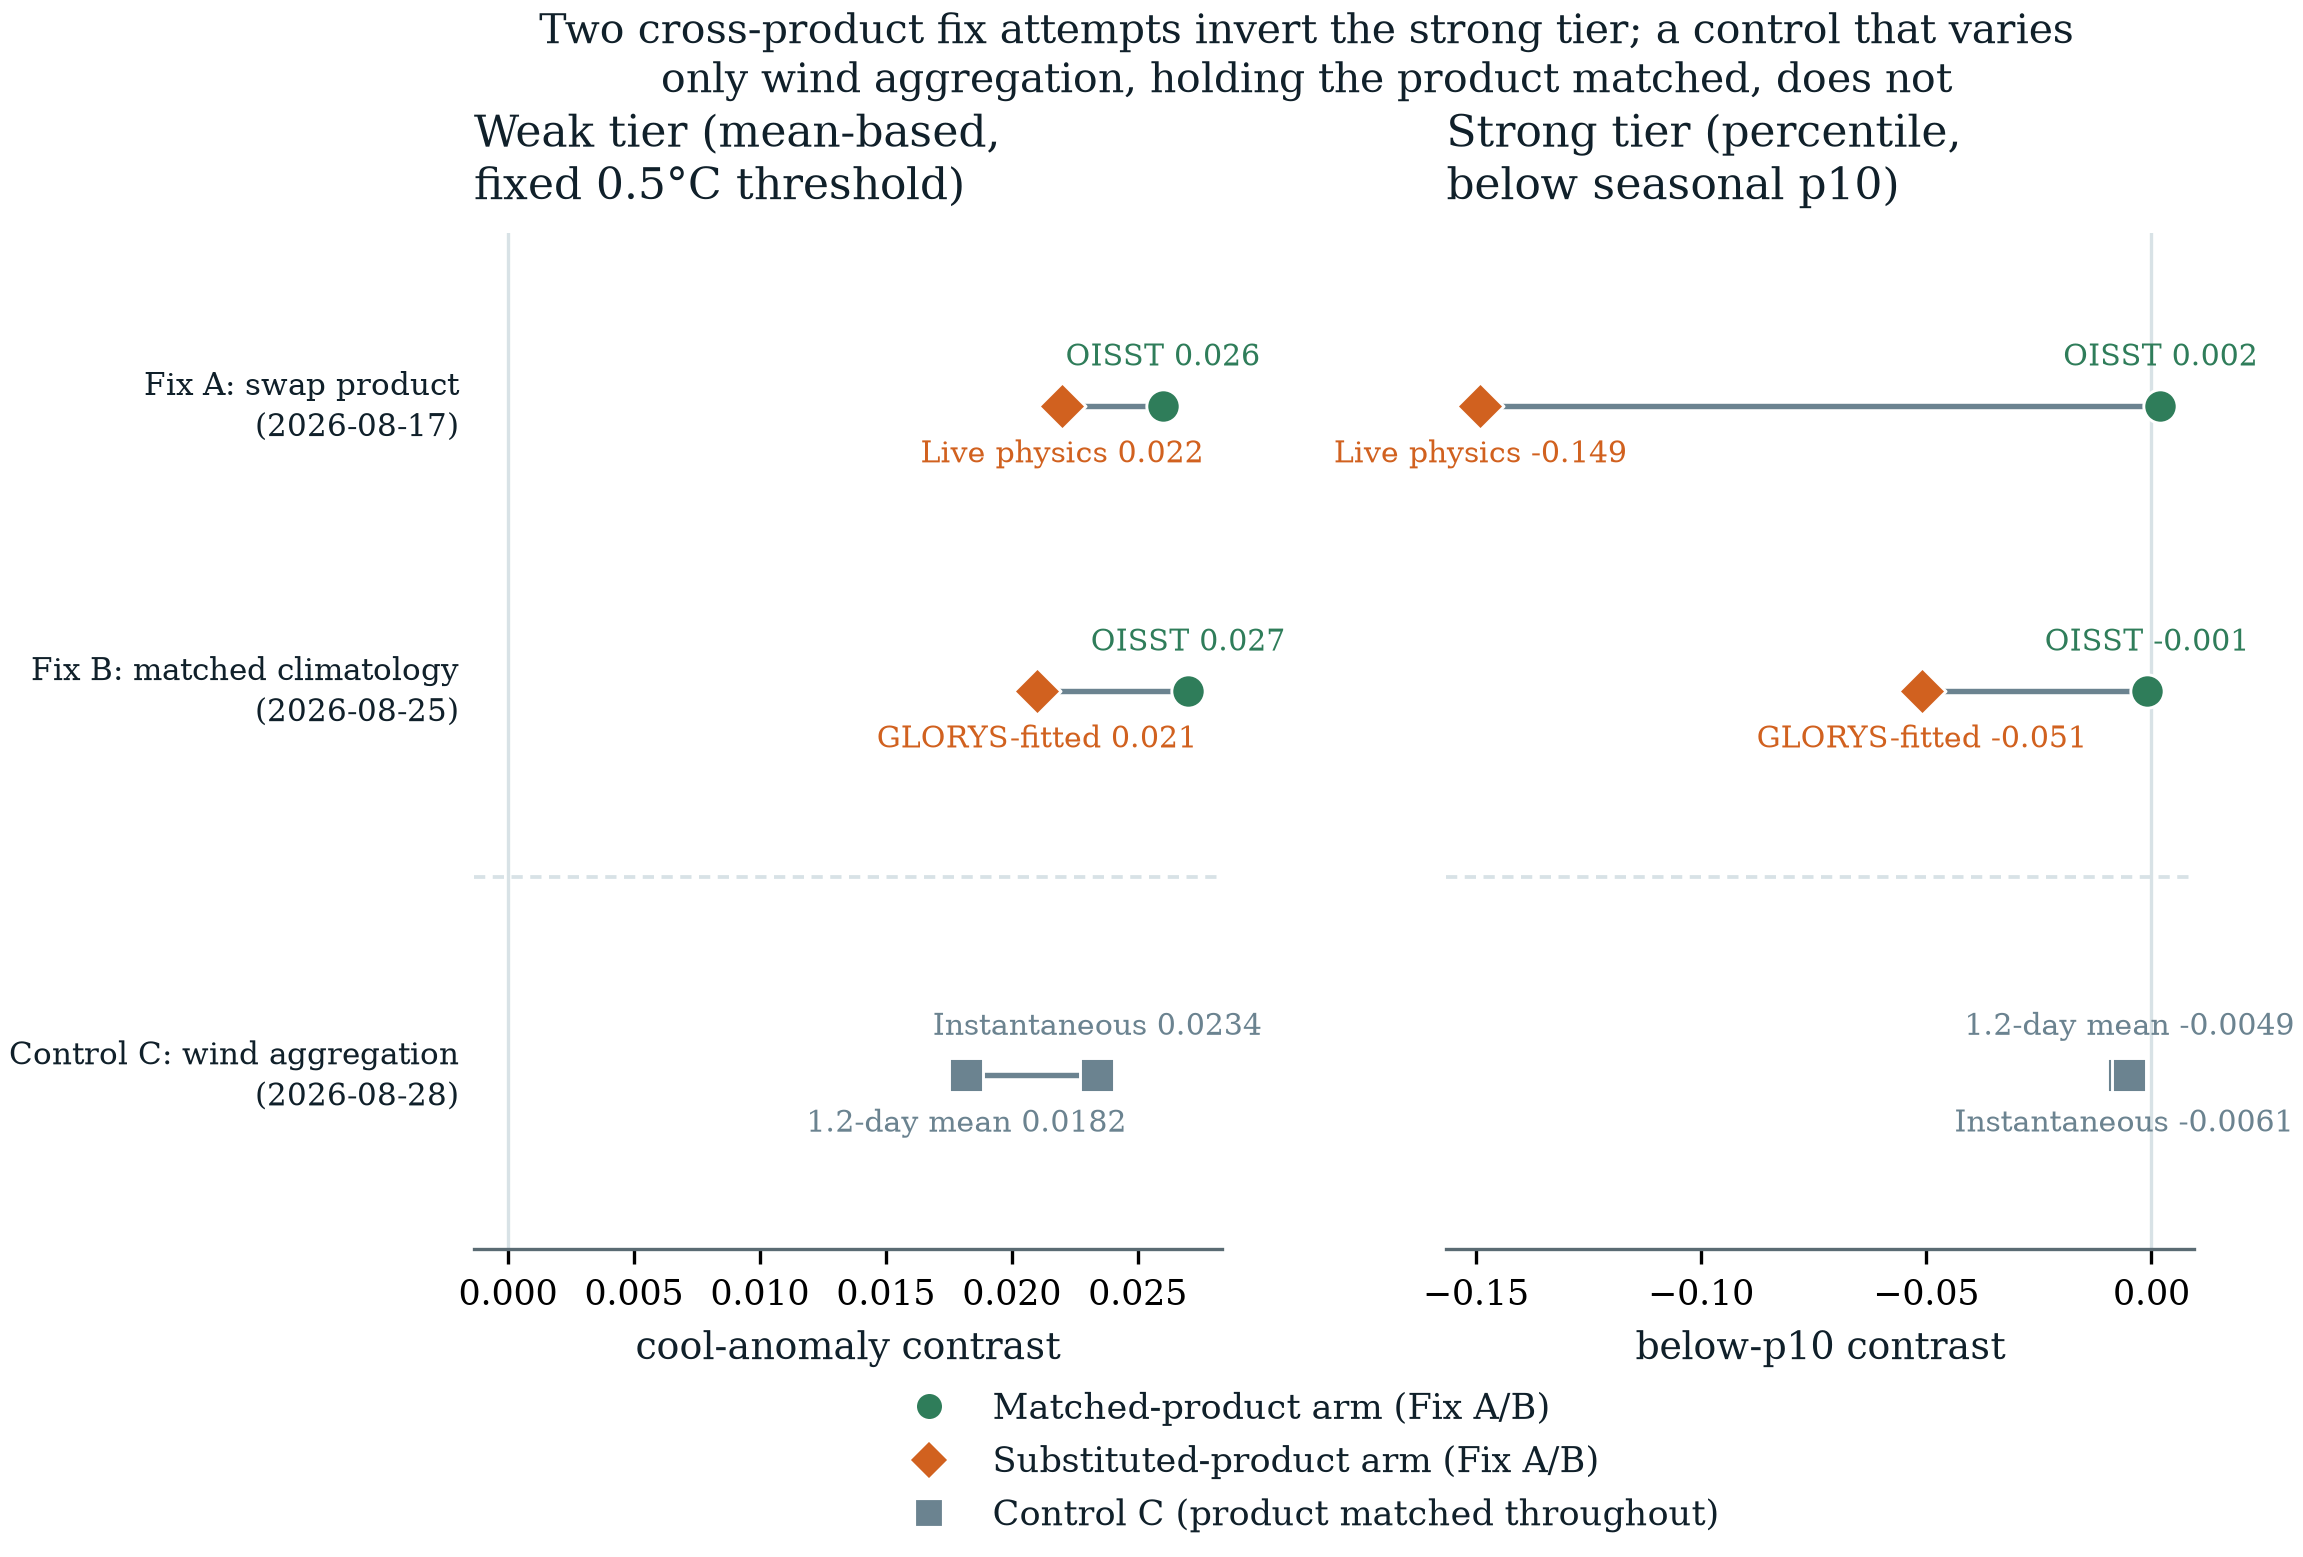
\includegraphics[width=0.92\linewidth]{fix_attempts}
\caption{The same six rows as Table~\ref{tab:fixes}, plotted as the arm each
attempt compares against its matched baseline. Left: the weak, mean-based
tier barely moves in any of the three attempts. Right: the strong,
percentile-based tier inverts sign in Fix A and Fix B (the two cross-product
substitutions) but stays near zero, same sign, in Control C (product held
matched throughout) -- visually separated from the first two rather than
grouped with them, because it answers a different question.}
\label{fig:fixes}
\end{wfigure}

\para{Fix A inverts the strong tier} Swapping the scored observation from
OISST to the live physics field, holding the climatology fixed, leaves the
weak tier essentially unchanged (\FixAWeakOisst{} against \FixAWeakLive{})
but moves the strong tier from a near-zero \FixAStrongOisst{} to
\FixAStrongLive{} --- downwelling-favourable (control) coastal cells came out
below their seasonal \ClimPercentile{}th percentile roughly three times as
often as favourable ones, the opposite of what the test is supposed to show.

\para{The cause is dispersion, not offset, and it concentrates on the coast}
The paired one-day comparison shows no systematic bias to correct: median
disagreement is \DisagOpenMedian{}\si{\celsius} in open water and
\DisagCoastalMedian{}\si{\celsius} across the coastal band --- both close to
zero, so a constant bias term would be a fudge with nothing to fix. What
differs sharply between the two is dispersion and mean: open-ocean cells show
a mean disagreement of \DisagOpenMean{}\si{\celsius} and standard deviation
\DisagOpenSD{}\si{\celsius}, with \DisagOpenFracHalf{}\% of cells differing by
more than \CoolAnomalyThreshold{}\si{\celsius} and \DisagOpenFracOne{}\% by more than a full
degree; the coastal band is worse on every one of those figures --- mean
\DisagCoastalMean{}\si{\celsius}, standard deviation \DisagCoastalSD{}\si{\celsius},
\DisagCoastalFracHalf{}\% and \DisagCoastalFracOne{}\% respectively. The
coastal standard deviation alone is wider than the \CoolAnomalyThreshold{}\si{\celsius}
threshold the weak tier is built around: a percentile tail test, whose
membership condition already sits close to a base rate of \(100 -
\ClimPercentile{}\)\% by construction, cannot survive noise the width of its
own signal, while a fixed-threshold test tolerates the same noise because the
threshold is large relative to the noise's mean effect on either side of the
comparison.

\para{Fix B does not rescue the tail test} Fitting the climatology on the
same product family as the live observation removes the cross-product
disagreement term measured above by construction --- the GLORYS-fitted
climatology and the live Copernicus physics field share a processing chain.
It does not rescue the strong tier: scored the same way on the same day, the
matched OISST arm reads \FixBWeakOisst{} weak / \FixBStrongOisst{} strong,
and the matched GLORYS arm reads \FixBWeakGlorys{} weak /
\FixBStrongGlorys{} strong --- the weak tier again barely moves, and the
strong tier again inverts, to a different but still substantially negative
value. Removing the specific \DisagCoastalSD{}\si{\celsius}-scale disagreement
Fix A's diagnosis pointed at was not sufficient; whatever destabilises the tail test
survives fitting a matched baseline.

\para{Control C rules out instantaneous sampling as the explanation} Holding
both the product and the climatology fixed at OISST-on-OISST throughout and
varying only the wind/currents field's temporal aggregation moves both
tiers, but only slightly, and in the same direction on both sides: weak
\CtrlWeakInstant{} to \CtrlWeakTrailing{}, strong \CtrlStrongInstant{} to
\CtrlStrongTrailing{}, a movement of \CtrlStrongDelta{} on the strong tier.
That is smaller than the \MatchedArmWander{} the matched arm's own strong-tier
value moved between Fix A's measurement date and Fix B's ---
run-to-run variation the matched configuration shows on its own, with nothing
about the wind input changed at all. Control C's contrasts stay the same sign
and close to zero in both arms; nothing in this measurement resembles Fix A's
or Fix B's inversion. This is evidence against instantaneous sampling being
what destabilises the tail test, which leaves the cross-product substitution
itself, demonstrated twice under two different attempted repairs, as the
explanation the data actually supports.

\section{Discussion}
\label{sec:discussion}

\para{Three measurements, two failures and one control, not three failures}
It would overstate this result to describe Control C as a third instance of
the same inversion: its own numbers do not invert, and its own reproduction
script states directly that it holds the SST source fixed at the one
production actually uses, varying only the wind. Its role is to close off the
most obvious objection to reading Fix A and Fix B as evidence of a genuine
product-mismatch effect rather than an artifact of scoring one instantaneous
field against another --- and by moving the contrast only slightly, in the
same direction on both arms, and by less than the matched arm's own
run-to-run wander, it does close that off. The honest structure of this
paper's result is two independently attempted, different-mechanism fixes for
the same underlying mismatch failing in the same qualitative way, plus a
control that rules out the leading alternative explanation for why.

\para{Why a tail test is more fragile than a mean-offset test} A fixed
absolute threshold on a mean-referenced anomaly and a seasonal percentile
threshold are both, in principle, ways of asking "is this cell unusually
cold." They differ in how close their decision boundary sits to the
distribution of plausible values. The weak tier's \CoolAnomalyThreshold{}\si{\celsius}
threshold is large relative to the corroboration signal being measured (a
contrast on the order of a few hundredths); injected, near-zero-median noise
of the measured dispersion perturbs cells near that boundary on both the
favourable and control sides by a similar amount, so the \emph{contrast} ---
already a difference of two small fractions --- moves little. The strong
tier's boundary is the seasonal \ClimPercentile{}th percentile, a threshold
defined to sit close to the edge of the baseline distribution by
construction; the coastal-band dispersion measured here
(\DisagCoastalSD{}\si{\celsius}) is comparable in scale to the climatological
gap between the mean and that percentile in the first place, so the same
injected noise can move a much larger share of cells across the boundary, in
either direction, than a mean-based threshold ever notices. This is a
property of the boundary's own tightness relative to the noise floor, not of
either product being wrong: OISST and the Copernicus physics products are
each defensible, quality-controlled estimates of the same physical quantity,
and the disagreement between them is ordinary product-to-product variation
of the kind the wider SST literature already documents \citep{reynolds2010}.
What is not ordinary, and not previously connected to that literature in this
form, is that the same variation degrades one class of downstream test
gracefully and destroys the other.

\para{A practical recipe} The two options this paper's own evidence supports
are not equally well demonstrated. Quoting the inter-product spread beside
the threshold --- reporting, alongside any percentile-based anomaly claim,
the dispersion between the product the climatology was fitted on and the
product the fresh observation actually came from --- costs one day of
overlapping data and is directly what \S\ref{sec:results}'s per-cell
comparison already does. Fitting the baseline on the product actually being
scored is the more complete fix in principle, but this paper's own Fix B
measurement is a demonstration that it is \emph{not sufficient on its own}:
the matched-product climatology removed the specific disagreement term
diagnosed after Fix A and the tail test still inverted. The recipe this
result supports is therefore the first option as a minimum bar for any
percentile-based claim scored across a product boundary, with matching the
baseline product as a partial mitigation whose own residual risk should be
re-measured, not assumed away, exactly as this paper had to do a second time
after Fix B did not close the gap Fix A opened.

\section{Limitations and Future Work}
\label{sec:limitations}

Every number in this paper is a single, dated, live measurement of a moving
field, and none is backed by a committed report or a passing regression
test; \S\ref{sec:methods}'s evidence grade says so explicitly and this
section repeats it because a result built entirely on dated numbers should
not be quietly read as more solid than that. Each of the three measurements
is one snapshot, not a repeated-sampling result: Control C's own docstring is
explicit that "this one run is a single snapshot at a
\WindHistoryWindowDays{}-day window, not a repeated-sampling result," and
does not rule out the originally targeted \WindHistoryTargetWindowDays{}-day
window or a different sampling scheme, only the specific window the real
backfill happened to obtain. The infrastructure to re-ask that question ---
\texttt{wind\_history.py}, \texttt{detect\_from\_history}, and the backfill
script --- is already built, which makes a longer window a re-run rather than
a re-build, but that re-run has not been done as of \AsOf{}.

This paper's scope is one region (the platform's coastal domain), one
variable (SST), and two source pairs (OISST/live-Copernicus-physics,
OISST/GLORYS-reanalysis). The general form this evidence points toward ---
that the substitution is safe up to a threshold approximately proportional to
the inter-product standard deviation, so a rule of the shape ``safe below
threshold \(\approx k \times\) inter-product sd'' could be stated and tested
--- has not been established here and is not established anywhere in this
platform's own research notes as of \AsOf{}; it remains exactly the open item
those notes already name, repeating this design across two or three further
product pairs and both tiers rather than the two pairs and the incidental
control measured here. Nothing in either attempted fix, or in the control
measurement, supersedes that open item; both fix attempts add a second and
third dated data point to the same single-region, single-variable case, not
a generalisation across it.

\section{Conclusion}

Scoring a fresh observation against a climatology fitted on a different data
product is treated, by the convention this practice runs on, as a
substitution that only affects timeliness. Measured directly inside a live
operational corroboration test, it is not: two independently attempted
fixes for the same underlying product mismatch --- swapping to a fresher,
higher-resolution live product, and fitting a matched climatology on the
product being scored --- both leave a weak, mean-based test of the same
signal nearly unchanged while inverting its strong, percentile-based tail
test, and a control measurement that varies only the wind input's temporal
aggregation rules out instantaneous sampling as an alternative explanation
for either. The cause is per-cell dispersion between the two products wider
than the decision threshold the weak tier tolerates and comparable in scale
to the climatological gap a percentile boundary is built close to. Every
number here is a dated, single measurement of a moving field, not a standing
fact, and the general rule this evidence points toward --- safe substitution
up to a threshold set by the inter-product spread --- remains to be
established across more than the two source pairs measured here.


\section*{Reproducibility}
Every number in this paper is graded \emph{Dated} in \S\ref{sec:methods}: a
single, live measurement of a moving field, reproducible on demand from a
committed script, with no stored output file backing any headline number.
{\raggedright\sloppy
Fix A and Fix B are reproduced by
\texttt{scripts/measure\_sst\_corroboration.py --source \{oisst,
copernicus\_reanalysis\}}; the GLORYS-fitted climatology Fix B scores against
is built by \texttt{scripts/build\_climatology\_copernicus.py}; the per-cell
disagreement measurement is read directly from
\texttt{services/sst\_anomaly.py}'s own module docstring. Control C is
reproduced by \texttt{scripts/measure\_wind\_history\_corroboration.py
--backfill-hours 72}, backfilling real wind history via
\texttt{scripts/backfill\_wind\_history.py} into
\texttt{services/wind\_history.py}.\par}
All five files are committed to the repository and were confirmed present as
of \AsOf{}; none of their outputs is.

\bibliographystyle{splncs04}
\bibliography{../shared/references}

\end{document}
